\documentclass[main.tex]{subfiles}

\begin{document}

\chapter{Simplicial sets}
\label{ch:simplicial_sets}

\section{Simplices as topological spaces and categories}
\label{sec:simplices_as_topological_spaces_and_categories}

One of the main themes in the study of higher category theory is the interplay between topology, simplicial geometry, and category theory.

\begin{equation*}
  \begin{aligned}
    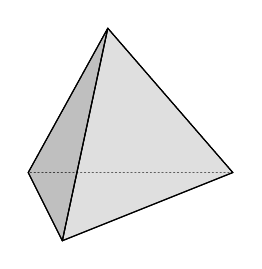
\begin{tikzpicture}[line join = round, scale=1.5, line cap = round]
      \coordinate (3) at (0,{sqrt(2)},0);
      \coordinate (2) at ({-.5*sqrt(3)},0,-.5);
      \coordinate (1) at (0,0,1);
      \coordinate (0) at ({.5*sqrt(3)},0,-.5);

      \draw[densely dotted,] (0)--(2);
      \draw[fill=lightgray,fill opacity=.5] (1)--(0)--(3)--cycle;
      \draw[fill=gray,fill opacity=.5] (2)--(1)--(3)--cycle;
      \draw (1)--(0);
      \draw (1)--(2);
      \draw (2)--(3);
      \draw (1)--(3);
      \draw (0)--(3);
    \end{tikzpicture}
  \end{aligned}
  \quad \longleftrightarrow \quad
  \begin{aligned}
    \begin{tikzpicture}[dot/.style={draw,circle,minimum size=1mm,inner sep=0pt,outer sep=0pt,fill=black}, line join = round, scale=1.5, line cap = round]

      \coordinate[draw, dot] (3) at (0,{sqrt(2)},0);
      \coordinate[draw, dot] (2) at ({.5*sqrt(3)},0,-.5);
      \coordinate[draw, dot] (1) at (0,0,1);
      \coordinate[draw, dot] (0) at ({-.5*sqrt(3)},0,-.5);

      \begin{scope}[decoration={markings,mark=at position 0.5 with {\arrow{to}}}]
        \draw[postaction={decorate}] (0)--(1);
        \draw[postaction={decorate}] (0)--(2);
        \draw[postaction={decorate}] (0)--(3);
        \draw[postaction={decorate}] (1)--(2);
        \draw[postaction={decorate}] (1)--(3);
        \draw[postaction={decorate}] (2)--(3);
      \end{scope}
    \end{tikzpicture}
  \end{aligned}
  \quad \longleftrightarrow \quad
  \begin{aligned}
    \begin{tikzcd}[row sep=tiny, column sep=tiny]
      && 2
      \arrow[drr]
      \\[2.5em]
      0
      \arrow[urr]
      \arrow[dr]
      \arrow[rrrr]
      &[5em]&&& 3
      \\[0.6em]
      & 1
      \arrow[urrr]
      \arrow[uur, crossing over]
    \end{tikzcd}
  \end{aligned}
\end{equation*}

The fundamental topological object we will study is the \emph{geometrical $n$-simplex.}

\begin{definition}[geometrical \texorpdfstring{$n$}{n}-simplex]
  \label{def:geometric_simplex}
  For any $n \geq 0$, the \defn{geometrical $n$-simplex}, denoted $\abs{\Delta^{n}}$, is the set (together with the subspace topology)
  \begin{equation*}
    \abs{\Delta^{n}} = \left\{(t_{0}, t_{1}, \ldots, t_{n}) \in \R^{n} \mid \sum_{i = 0}^{n} t_{i} = 1 \text{ and } t_{i} \geq 0 \text{ for all }i \right\}.
  \end{equation*}
\end{definition}

In simplicial geometry, one replaces these topological models of simplices by combinatorial models of simplices. These live in a category.

\begin{definition}[simplex category]
  \label{def:simplex_category}
  Denote by $\Delta$ the category whose objects are linearly ordered sets
  \begin{equation*}
    [n] = \{0, \ldots, n\}
  \end{equation*}
  and whose morphisms $n \to m$ are weakly monotonic\footnote{i.e.\ nondecreasing in the sense that $i \geq j \implies f(i) \geq f(j)$} maps.
\end{definition}

The objects $[n]$ of $\Delta$ are to be interpreted as simplices with ordered vertices. For example,
\begin{equation*}
  [0] =
  \begin{aligned}
    \begin{tikzpicture}[dot/.style={draw,circle,minimum size=1mm,inner sep=0pt,outer sep=0pt,fill=black}, scale=1.5]
      \coordinate[draw, dot];
    \end{tikzpicture}
  \end{aligned}
  \,,\qquad [1] =
  \begin{aligned}
    \begin{tikzpicture}[dot/.style={draw,circle,minimum size=1mm,inner sep=0pt,outer sep=0pt,fill=black}, scale=1.5]
      \coordinate[draw, dot] (0) at (0,0);
      \coordinate[draw, dot] (1) at (1,0);

      \begin{scope}[decoration={markings,mark=at position 0.5 with {\arrow{to}}}]
        \draw[postaction={decorate}] (0)--(1);
      \end{scope}
    \end{tikzpicture}
  \end{aligned}
  \,,\qquad [2] =
  \begin{aligned}
    \begin{tikzpicture}[dot/.style={draw,circle,minimum size=1mm,inner sep=0pt,outer sep=0pt,fill=black}, scale=1.5]
      \coordinate[draw, dot] (0) at (0,0);
      \coordinate[draw, dot] (1) at (0.5,0.7);
      \coordinate[draw, dot] (2) at (1,0);

      \begin{scope}[decoration={markings,mark=at position 0.5 with {\arrow{to}}}]
        \draw[postaction={decorate}] (0)--(1);
        \draw[postaction={decorate}] (0)--(2);
        \draw[postaction={decorate}] (1)--(2);
      \end{scope}
    \end{tikzpicture}
  \end{aligned}
  \,, \qquad [3] =
  \begin{aligned}
    \begin{tikzpicture}[dot/.style={draw,circle,minimum size=1mm,inner sep=0pt,outer sep=0pt,fill=black}, line join = round, scale=1, line cap = round]

      \coordinate[draw, dot] (3) at (0,{sqrt(2)},0);
      \coordinate[draw, dot] (2) at ({.5*sqrt(3)},0,-.5);
      \coordinate[draw, dot] (1) at (0,0,1);
      \coordinate[draw, dot] (0) at ({-.5*sqrt(3)},0,-.5);

      \begin{scope}[decoration={markings,mark=at position 0.5 with {\arrow{to}}}]
        \draw[postaction={decorate}] (0)--(1);
        \draw[postaction={decorate}] (0)--(2);
        \draw[postaction={decorate}] (0)--(3);
        \draw[postaction={decorate}] (1)--(2);
        \draw[postaction={decorate}] (1)--(3);
        \draw[postaction={decorate}] (2)--(3);
      \end{scope}
    \end{tikzpicture}
  \end{aligned}
\end{equation*}

We can connect our simplex category to geometric simplices using a functor.

\begin{definition}[realization functor]
  \label{def:realization_functor}
  The \defn{realization functor}
  \begin{equation*}
    \rho\colon \Delta \to \mathbf{Top}
  \end{equation*}
  is defined on objects by $[n] \mapsto \abs{\Delta^{n}}$ and on morphisms $[f]\colon [m] \to [n]$ by
  \begin{equation*}
    f_{*}\colon \abs{\Delta^{m}} \to \abs{\Delta^{n}};\qquad (t_{0}, \ldots, t_{m}) \mapsto (s_{1}, \ldots, s_{m}),
  \end{equation*}
  where
  \begin{equation*}
    s_{i} =
    \begin{cases}
      0, & f^{-1}(i) = \emptyset \\
      \sum_{j \in J^{-1}(i)} t_{j} & \text{otherwise.}
    \end{cases}
  \end{equation*}
\end{definition}
That is, $\rho$ assigns to each combinatorial $n$-simplex its topological counterpart.
\begin{equation*}
  \rho:\quad
  \begin{aligned}
    \begin{tikzpicture}[dot/.style={draw,circle,minimum size=1mm,inner sep=0pt,outer sep=0pt,fill=black}, line join = round, scale=1.5, line cap = round]

      \coordinate[draw, dot] (3) at (0,{sqrt(2)},0);
      \coordinate[draw, dot] (2) at ({.5*sqrt(3)},0,-.5);
      \coordinate[draw, dot] (1) at (0,0,1);
      \coordinate[draw, dot] (0) at ({-.5*sqrt(3)},0,-.5);

      \begin{scope}[decoration={markings,mark=at position 0.5 with {\arrow{to}}}]
        \draw[postaction={decorate}] (0)--(1);
        \draw[postaction={decorate}] (0)--(2);
        \draw[postaction={decorate}] (0)--(3);
        \draw[postaction={decorate}] (1)--(2);
        \draw[postaction={decorate}] (1)--(3);
        \draw[postaction={decorate}] (2)--(3);
      \end{scope}
    \end{tikzpicture}
  \end{aligned}
  \quad \longmapsto \quad
  \begin{aligned}
    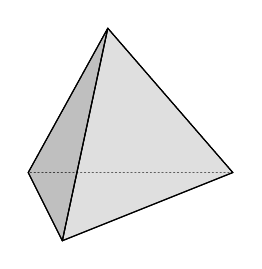
\begin{tikzpicture}[line join = round, scale=1.5, line cap = round]
      \coordinate (3) at (0,{sqrt(2)},0);
      \coordinate (2) at ({-.5*sqrt(3)},0,-.5);
      \coordinate (1) at (0,0,1);
      \coordinate (0) at ({.5*sqrt(3)},0,-.5);

      \draw[densely dotted,] (0)--(2);
      \draw[fill=lightgray,fill opacity=.5] (1)--(0)--(3)--cycle;
      \draw[fill=gray,fill opacity=.5] (2)--(1)--(3)--cycle;
      \draw (1)--(0);
      \draw (1)--(2);
      \draw (2)--(3);
      \draw (1)--(3);
      \draw (0)--(3);
    \end{tikzpicture}
  \end{aligned}
\end{equation*}

One can also think of these combinatorial simplices categorically. Again, this connection is given by a functor.

\begin{definition}[categorification functor]
  \label{def:categorification_functor}
  The \defn{categorification functor} is the functor
  \begin{equation*}
    \chi\colon \Delta \to \mathbf{Cat}
  \end{equation*}
  which sends the object $[n]$ to the poset category on $[n]$. Note that functors $[m] \to [n]$ are the same thing as weakly monotonic maps $[m] \to [n]$.
\end{definition}

That is, $\chi$ assigns to each combinatorial $n$-simplex its categorical counterpart.
\begin{equation*}
  \chi\colon \quad
  \begin{aligned}
    \begin{tikzpicture}[dot/.style={draw,circle,minimum size=1mm,inner sep=0pt,outer sep=0pt,fill=black}, line join = round, scale=1.5, line cap = round]

      \coordinate[draw, dot] (3) at (0,{sqrt(2)},0);
      \coordinate[draw, dot] (2) at ({.5*sqrt(3)},0,-.5);
      \coordinate[draw, dot] (1) at (0,0,1);
      \coordinate[draw, dot] (0) at ({-.5*sqrt(3)},0,-.5);

      \begin{scope}[decoration={markings,mark=at position 0.5 with {\arrow{to}}}]
        \draw[postaction={decorate}] (0)--(1);
        \draw[postaction={decorate}] (0)--(2);
        \draw[postaction={decorate}] (0)--(3);
        \draw[postaction={decorate}] (1)--(2);
        \draw[postaction={decorate}] (1)--(3);
        \draw[postaction={decorate}] (2)--(3);
      \end{scope}
    \end{tikzpicture}
  \end{aligned}
  \quad \longmapsto \quad
  \begin{aligned}
    \begin{tikzcd}[row sep=tiny, column sep=tiny]
      && 2
      \arrow[drr]
      \\[2.5em]
      0
      \arrow[urr]
      \arrow[dr]
      \arrow[rrrr]
      &[5em]&&& 3
      \\[0.6em]
      & 1
      \arrow[urrr]
      \arrow[uur, crossing over]
    \end{tikzcd}
  \end{aligned}
\end{equation*}

These categories and functors may seem too simple to be of any real use, but one can build astonishingly complicated structures out of them.

\section{Simplicial sets}
\label{sec:simplicial_sets}

A simplicial set is thought of as a collection of standard simplices of various degrees, glued together along their faces. That is, a simplicial set consists of, for each $n \in \N$, a collection of simplices of degree $n$, together with rules for how to glue them together. This data can be specified efficiently in the following way.

\begin{definition}[simplicial set]
  \label{def:simplicial_set}
  A \defn{simplicial set} is a functor $\Delta\op \to \mathbf{Set}$. The category of simplicial sets is the category of such functors, i.e.\
  \begin{equation*}
    \mathbf{Cat}(\Delta\op, \mathbf{Set}) = \SSet.
  \end{equation*}
\end{definition}

As discussed briefly in \hyperref[sec:yoneda_extensions]{Section~\ref*{sec:yoneda_extensions}}, one thinks of the image under the Yoneda embedding of the object $[n]$ as an $n$-simplex, called the \emph{standard $n$-simplex,} and more general simplicial sets as being built by gluing standard simplices together.

Specifically, for any simplicial set $K$ we should interpret $K([n])$ as the set of $n$-simplices contained in $K$. The gluing conditions come from functoriality. We will investigate this in \hyperref[sec:what_sort_of_data_does_a_simplicial_set_give_us]{Section~\ref*{sec:what_sort_of_data_does_a_simplicial_set_give_us}}.

\begin{definition}[standard simplex]
  \label{eg:standard_simplex}
  Let $n \geq 0$. The simplicial set
  \begin{equation*}
    \Delta(-, [n]) = \mathcal{Y}([n])
  \end{equation*}
  is denoted $\Delta^{n}$, and called the \emph{standard $n$-simplex.}
\end{definition}

The claim is that the standard $n$-simplex can be interpreted geometrically, as precisely the sort of picture we have been drawing. To see this, it will be helpful to explicitly analyze some cases in which $n$ is small. Take $n = 2$. To justify the name, the standard $2$-simplex had better look something like the 2-simplex we know and love.
\begin{equation*}
  \begin{tikzpicture}[dot/.style={draw,circle,minimum size=1mm,inner sep=0pt,outer sep=0pt,fill=black}, scale=2]
    \coordinate[draw, dot, label=210:0] (0) at (0,0);
    \coordinate[draw, dot, label=90:1] (1) at (0.5,0.7);
    \coordinate[draw, dot, label=-30:2] (2) at (1,0);

    \begin{scope}[decoration={markings,mark=at position 0.5 with {\arrow{to}}}]
      \draw[postaction={decorate}] (0)--(1);
      \draw[postaction={decorate}] (0)--(2);
      \draw[postaction={decorate}] (1)--(2);
    \end{scope}
  \end{tikzpicture}
\end{equation*}
Specifically, we should interpret $\Delta^{2}([n])$ as the set of $n$-simplices contained in $\Delta^{2}$. Naïvely, we would expect three 0-simplices, three 1-simplices, and one 2-simplex.

However, the only way to find out what we actually have is to begin calculating. First, we calculate $\Delta^{2}([0]) = \SSet([0], [2])$:
\begin{equation*}
  \Delta^{2}([0]) = \{0 \mapsto 0, 0 \mapsto 1, 0 \mapsto 2\}.
\end{equation*}
To avoid formulae whose lengths quickly get out of hand, we will drop the functional notation, denoting the above by $\{0, 1, 2\}$.

This is good. We said that $\Delta^{2}([0])$ should be interpreted as the set of 0-simplices, and indeed $\Delta^{2}([0])$ has three elements, which represent in an obvious way the vertices of the familiar 2-simplex. Now calculating $\Delta^{2}([1])$, we find
\begin{equation*}
  \Delta^{2}([1]) = \{\{0,1\} \mapsto \{0,1\}, \{0,2\}, \{1,2\}, \{0,0\}, \{1,1\}, \{2,2\}\}.
\end{equation*}
This is not so good; we can interpret the three edges $\{0, 1\}$, $\{0, 2\}$, and $\{1, 2\}$ as the edges between 0 and 1, 0 and 2, and 1 and 2 that we were expecting, but we also have three more. We interpret these as `degenerate edges,' which are all bunched up at the vertices. This is one difference between simplicial complexes and simplicial sets: simplicial sets can have degenerate edges.

Continuing, we find
\begin{equation*}
  \Delta^{2}([2]) = \{\{0,0,0\}, \{0,0,1\}, \{0,0,2\}, \ldots\}.
\end{equation*}
We recognize these as degenerate faces. The only nondegenerate face will be $\{0,1,2\}$.

Note that contrary to what you might expect, $\Delta^{n}([k])$ is not empty for $k > n$; it is simply filled with an enormous number of degenerate simplices.\footnote{To be precise, with $\begin{pmatrix} n+k+1 \\ k \end{pmatrix}$ simplices.}

\begin{example}
  Denote the power set of a set $X$ by $\mathcal{P}(X)$. Let $\mathcal{J} \subseteq \mathcal{P}(\{0, 1, \ldots, n\})$. Then there is a simplicial set $\Delta^{\mathcal{J}}$ whose morphisms are defined to be the subset
  \begin{equation*}
    \Delta^{\mathcal{J}}([n]) \subseteq \Delta([m], [n])
  \end{equation*}
  consisting of those $f$ such that $\mathrm{im}(f) \subset J$ for some $J \in \mathcal{J}$.

  Here are some specific examples of $\mathcal{J}$ which will be useful to us. \begin{itemize}
    \item If $\mathcal{J} = \mathcal{P}(\{0, \ldots, n\})$, then
      \begin{equation*}
        \Delta^{\mathcal{J}}([n]) = \Delta^{n},
      \end{equation*}
      the standard $n$-simplex.

    \item If
      \begin{equation*}
        \mathcal{J} = \mathcal{P}(\{0, 1, \ldots, n\}) \smallsetminus \{\{0, 1, \ldots, n\}\},
      \end{equation*}
      then the simplicial set we obtain is called the \emph{boundary} of $\Delta^{n}$, and denoted $\partial \Delta^{n}$.

      The sets $\Delta^{n}([i])$ and $\partial \Delta^{n}([i])$ are the same for $i < n$. 

    \item Fix some $i$ such that $0 \leq i \leq n$. Then with
      \begin{equation*}
        \mathcal{J} = \mathcal{P}(\{0, 1, \ldots, n\}) \smallsetminus \{\{0, 1, \ldots, n\}, \{0, 1, \ldots, i - 1, i + 1, \ldots, n\}\},
      \end{equation*}
      we obtain the \emph{$i$th horn} of $\Delta^{n}$, and denoted $\Lambda^{n}_{i}$.

      For example, the $2$-simplices in the horn $\Lambda^{2}_{1}$ consists of the subset of monotone functions $[2] \to [2]$ whose range lies entirely within one of the sets $\{0,1,2,01, 12, 22\}$. That is
      \begin{equation*}
        \{000, 001, 011, 111, 112, 122, 222\}.
      \end{equation*}
      We can draw $\Lambda^{2}_{i}$, for $i = 0$, $1$, $2$, as follows.
      \begin{equation*}
        \Lambda^{2}_{0} =
        \begin{aligned}
          \begin{tikzpicture}[dot/.style={draw,circle,minimum size=1mm,inner sep=0pt,outer sep=0pt,fill=black}, scale=2]
            \coordinate[draw, dot, label=210:0] (0) at (0,0);
            \coordinate[draw, dot, label=90:1] (1) at (0.5,0.7);
            \coordinate[draw, dot, label=-30:2] (2) at (1,0);

            \begin{scope}[decoration={markings,mark=at position 0.5 with {\arrow{to}}}]
              \draw[postaction={decorate}] (0)--(1);
              \draw[postaction={decorate}] (0)--(2);
            \end{scope}
          \end{tikzpicture}
        \end{aligned}
        ,\qquad \Lambda^{2}_{1} =
        \begin{aligned}
          \begin{tikzpicture}[dot/.style={draw,circle,minimum size=1mm,inner sep=0pt,outer sep=0pt,fill=black}, scale=2]
            \coordinate[draw, dot, label=210:0] (0) at (0,0);
            \coordinate[draw, dot, label=90:1] (1) at (0.5,0.7);
            \coordinate[draw, dot, label=-30:2] (2) at (1,0);

            \begin{scope}[decoration={markings,mark=at position 0.5 with {\arrow{to}}}]
              \draw[postaction={decorate}] (0)--(1);
              \draw[postaction={decorate}] (1)--(2);
            \end{scope}
          \end{tikzpicture}
        \end{aligned}
        ,\qquad \Lambda^{2}_{2} =
        \begin{aligned}
          \begin{tikzpicture}[dot/.style={draw,circle,minimum size=1mm,inner sep=0pt,outer sep=0pt,fill=black}, scale=2]
            \coordinate[draw, dot, label=210:0] (0) at (0,0);
            \coordinate[draw, dot, label=90:1] (1) at (0.5,0.7);
            \coordinate[draw, dot, label=-30:2] (2) at (1,0);

            \begin{scope}[decoration={markings,mark=at position 0.5 with {\arrow{to}}}]
              \draw[postaction={decorate}] (0)--(2);
              \draw[postaction={decorate}] (1)--(2);
            \end{scope}
          \end{tikzpicture}
        \end{aligned}
      \end{equation*}
  \end{itemize}
\end{example}

\begin{definition}[inner, outer horn]
  \label{def:inner_outer_horn}
  If $i = 0$ or $i = n$, then we say that $\Delta^{n}_{i}$ is an \defn{outer horn}. Otherwise, if $0 < i < n$, we say that $\Lambda^{n}_{i}$ is an \defn{inner horn}.
\end{definition}

\begin{definition}[simplicial complex]
  \label{def:simplicial_complex}
  A set $\mathcal{K} \subset \mathcal{P}(\{0, 1, \ldots, n\})$ is called an \defn{simplicial complex} if for every $\mathcal{J} \in \mathcal{K}$ and $I \subseteq \mathcal{J}$ with $I \neq \emptyset$, $I \in \mathcal{K}$.
\end{definition}

\begin{example}
  Let $\mathcal{K}$ be any simplicial complex. We can interpret $\mathcal{K}$ as a simplicial set by associating
  \begin{equation*}
    \mathcal{K} \mapsto \Delta^{\mathcal{K}}.
  \end{equation*}
  What would have been called the simplices of $\mathcal{K}$ correspond to the nondegenerate elements of the simplicial complex. Note however that there are many simplicial sets which are not obtained from simplicial complexes in this way.
\end{example}

Simplicial sets are functors, but the functorial notation is often unnecessarily burdensome. Therefore, it is standard to denote the $n$-simplices of a simplicial set $K$ by $K_{n}$ rather than $K([n])$. This is the notation that we will use from now on unless it will be confusing.

\section{What sort of data does a simplicial set give us?}
\label{sec:what_sort_of_data_does_a_simplicial_set_give_us}

Let $K$ be a simplicial set. We have seen that evaluating $K$ on the object $[n]$ gives a set, which we interpret as the set of $n$-simplices making up $K$. We have claimed that the functoriality of $K$ provides instructions for how these simplices should be glued together. In this section we will investigate this claim.

First, we note that we can understand how $K$ acts on morphisms $\phi\colon [n] \to [m]$ by understanding how it behaves on simpler functions, known as the \emph{face} and \emph{degeneracy functions.}

\begin{definition}[degeneracy function]
  \label{def:degeneracy_function_simplicial_category}
  Let $n > 0$. For every $i$ with $0 \leq i \leq n$, there is a function
  \begin{equation*}
    \sigma_{k}\colon [n] \to [n - 1];\qquad j \mapsto
    \begin{cases}
      j, & j \leq k \\
      j - 1, & j > k
    \end{cases}
  \end{equation*}
  called the \defn{$i$th degeneracy function}.
\end{definition}
\begin{equation*}
  \sigma_{k} \quad = \quad
  \begin{tikzcd}[row sep=tiny]
    \vdots & \vdots
    \\
    k-2
    \arrow[r, mapsto]
    & k-2
    \\
    k-1 
    \arrow[r, mapsto]
    & k-1
    \\
    k 
    \arrow[r, mapsto]
    & k
    \\
    k+1 
    \arrow[ur, mapsto]
    & k+1
    \\
    k+2
    \arrow[ur, mapsto]
    & k+2
    \\
    \vdots & \vdots
  \end{tikzcd}
\end{equation*}

\begin{definition}[face function]
  \label{def:face_function_simplicial_category}
  Let $n \geq 0$. For any $k$ with $0 \leq k < n$, there is a function
  \begin{equation*}
    \partial_{i}\colon [n - 1] \to [n];\qquad j \to
    \begin{cases}
      j, & j < i \\
      j + 1, & j \geq i
    \end{cases}
  \end{equation*}
  called the \defn{$i$th face function}.
\end{definition}
\begin{equation*}
  \sigma_{k} \quad = \quad
  \begin{tikzcd}[row sep=tiny]
    \vdots & \vdots
    \\
    k-2
    \arrow[r, mapsto]
    & k-2
    \\
    k-1 
    \arrow[r, mapsto]
    & k-1
    \\
    k 
    \arrow[r, mapsto]
    & k
    \\
    k+1 
    \arrow[dr, mapsto]
    & k+1
    \\
    k+2
    \arrow[dr, mapsto]
    & k+2
    \\
    \vdots & \vdots
  \end{tikzcd}
\end{equation*}

If we were being pedantic, we would denote these functions $\sigma^{n}_{k}$ and $\partial^{n}_{i}$ instead of $\sigma_{k}$ and $\partial_{i}$, but keeping track of these indices turns out to be more confusing than elucidating, so no one does.

The face and degeneracy functions are interesting because they generate all morphisms; that is, any morphism $\phi\colon [n] \to [m]$ can be written as a composition of face and degeneracy functions.

\begin{proposition}
  Let $\phi\colon [n] \to [m]$ be a weakly monotonic function. Then $\phi$ can be written as a composition of face and degeneracy maps.
\end{proposition}
\begin{proof}[Sketch of proof]
  Since $\phi$ is by definition nondecreasing, we can specify it by, starting from $0$, a sequence 
\end{proof}

\begin{definition}[degeneracy map]
  \label{def:degeneracy_map}
  Let $X\colon \Delta\op \to \mathbf{Set}$ be a simplicial set. Corresponding to the degeneracy function $\sigma_{k}\colon [n] \to [n-1]$ there is a corresponding map
  \begin{equation*}
    s_{k}\colon X_{n-1} \to X_{n}.
  \end{equation*}
  This map is also known as the \defn{$k$th degeneracy map}.
\end{definition}

\begin{definition}[face map]
  \label{def:face_map}
  Let $X\colon \Delta\op \to \mathbf{Set}$ be a simplicial set. Corresponding to the face function $\partial_{i}\colon [n] \to [n-1]$ (see \hyperref[def:face_function_simplicial_category]{Definition~\ref*{def:face_function_simplicial_category}}), there is a map
  \begin{equation*}
    d_{i}\colon X_{n} \to X_{n-1}.
  \end{equation*}
  This map is also known as the \defn{$i$th face map}.
\end{definition}
\begin{example}
  Consider the simplicial set $\Delta^{2}$, and the map
  \begin{equation*}
    d_{0}\colon \Delta^{2}_{1} \to \Delta^{2}_{0}.
  \end{equation*}
  Let $f \in \Delta^{2}_{1} = \Delta([1], [2])$. For example, take
  \begin{equation*}
    f\colon\quad
    \begin{tikzcd}[row sep=tiny]
      0
      \arrow[mapsto, dr]
      & 0
      \\
      1
      \arrow[mapsto, rd]
      & 1
      \\
      & 2
    \end{tikzcd}
  \end{equation*}
  corresponding to the solid edge.
  \begin{equation*}
    \begin{tikzpicture}[dot/.style={draw,circle,minimum size=1mm,inner sep=0pt,outer sep=0pt,fill=black}, scale=2]
      \coordinate[label=210:0] (0) at (0,0);
      \coordinate[draw, dot, label=90:1] (1) at (0.5,0.7);
      \coordinate[draw, dot, label=-30:2] (2) at (1,0);

      \begin{scope}[decoration={markings,mark=at position 0.5 with {\arrow{to}}}]
        \draw[dashed, postaction={decorate}] (0)--(1);
        \draw[dashed, postaction={decorate}] (0)--(2);
        \draw[postaction={decorate}] (1)--(2);
      \end{scope}
    \end{tikzpicture}
  \end{equation*}
  Which element of $\Delta^{2}_{0}$ does $d_{0}$ send this to? We can draw $\partial_{0}$ like this.
  \begin{equation*}
    \partial_{0}\colon \quad
    \begin{tikzcd}[row sep=tiny]
      0
      \arrow[mapsto, rd]
      & 0
      \\
      & 1
    \end{tikzcd}
  \end{equation*}
  The map $d_{0}$ acts by precomposing with $\partial_{0}$.
  \begin{equation*}
    d_{0}f = f \circ \partial_{0} = \quad
    \begin{tikzcd}[row sep=tiny]
      0
      \arrow[mapsto, dr]
      & 0
      \arrow[mapsto, dr]
      & 0
      \\
      & 1
      \arrow[dr, mapsto]
      & 1
      \\
      && 2
    \end{tikzcd}
    \quad = \quad
    \begin{tikzcd}[row sep=tiny]
      0
      \arrow[rdd, mapsto]
      & 0
      \\
      & 1
      \\
      & 2
    \end{tikzcd}
  \end{equation*}

  Therefore, $d_{0}$ takes the edge between $0$ and $2$ to the vertex $2$.
  \begin{equation*}
    \begin{tikzpicture}[dot/.style={draw,circle,minimum size=1mm,inner sep=0pt,outer sep=0pt,fill=black}, scale=2]
      \coordinate[label=210:0] (0) at (0,0);
      \coordinate[label=90:1] (1) at (0.5,0.7);
      \coordinate[draw, dot, label=-30:2] (2) at (1,0);

      \begin{scope}[decoration={markings,mark=at position 0.5 with {\arrow{to}}}]
        \draw[dashed, postaction={decorate}] (0)--(1);
        \draw[dashed, postaction={decorate}] (0)--(2);
        \draw[dashed, postaction={decorate}] (1)--(2);
      \end{scope}
    \end{tikzpicture}
  \end{equation*}

  Similarly, $d_{0}$ takes the edge between $0$ and $1$ to the vertex $1$, and the full 2-simplex to the edge between 1 and 2.
\end{example}

This is a general feature: the $i$th face $d_{i}$ map deletes the $i$th vertex.

\begin{theorem}[simplicial identites]
  \label{thm:simplicial_identities}
  The face maps and degeneracy maps satisfy the following conditions, known as the \emph{simplicial identities.}
  \begin{align*}
    d_{i} \circ d_{j} &= d_{j - 1} \circ d_{i},&i < j \\
    d_{i} \circ s_{j} &= s_{j-1} \circ d_{i}, &i < j \\
    d_{j} \circ s_{j} &= 1 = d_{j+1} \circ s_{j} \\
    d_{i} \circ s_{j} &= s_{j} \circ d_{i-1}, &i > j + 1 \\
    s_{i} \circ s_{j} &= s_{j+1} \circ s_{i}, &i \leq j.
  \end{align*}
\end{theorem}

\begin{corollary}
  We have immediately that
  \begin{equation*}
    d_{i} \circ d_{j} = d_{j} \circ d_{i+1},\qquad i+1 > j.
  \end{equation*}
\end{corollary}

\begin{fact}
  The definition of a simplicial set is equivalent to the definition the following data.
  \begin{itemize}
    \item The sets $X_{n}$, $n \geq 0$.
    \item The face and degeneracy maps satisfying the simplicial identities.
  \end{itemize}
\end{fact}

\section{Basic properties of the category of simplicial sets}
\label{sec:basic_properties_of_the_category_of_simplicial_sets}

The category of simplicial sets is a category of functors whose codomain is $\mathbf{Set}$. Any functor category inherits a lot of structure from it codomain category. In the case of $\SSet$, the category $\mathbf{Set}$ has an enormous amount of structure. In this section we list some of the structure $\SSet$ inherits from $\Set$.

\subsection{Existence of limits and colimits}
\label{ssc:existence_of_limits_and_colimits}

\begin{proposition}
  \label{prop:sset_has_limits_colimits}
  The category $\SSet$ has small limits and colimits, which are computed pointwise.
\end{proposition}
\begin{proof}
  The category $\mathbf{Set}$ has small limits and colimits, which implies by \hyperref[thm:functor_categories_complete_cocomplete]{Theorem~\ref*{thm:functor_categories_complete_cocomplete}} that any functor category $\mathrm{Fun}(\mathcal{C}, \mathbf{Set})$ does.

  Limits and colimits are computed pointwise thanks to \hyperref[cor:monos_epis_in_functor_category_preserved_pointwise]{Corollary~\ref*{cor:monos_epis_in_functor_category_preserved_pointwise}}.
\end{proof}

\begin{example}[products]
  By \hyperref[cor:limits_computed_pointwise]{Corollary~\ref*{cor:limits_computed_pointwise}}, we can compute this limit pointwise; that is
  \begin{equation*}
    (X \times Y)_{n} = X_{n} \times Y_{n}.
  \end{equation*}

  Let us understand this this by studying $\Delta^{1} \times \Delta^{1}$ in some detail.

  The 0-simplices of $\Delta^{1} \times \Delta^{1}$ are ordered pairs $\Delta^{1}_{0} \times \Delta^{1}_{0} = \{0, 1\} \times \{0, 1\}$. We can visualize this like so.
  \begin{equation*}
    \begin{tikzpicture}[dot/.style={draw,circle,minimum size=1mm,inner sep=0pt,outer sep=0pt,fill=black}, scale=2]
      \coordinate[draw, dot, label=left:${(0, 0)}$] (00) at (0,0);
      \coordinate[draw, dot, label=left:${(0, 1)}$] (01) at (0,1);
      \coordinate[draw, dot, label=right:${(1, 0)}$] (10) at (1,0);
      \coordinate[draw, dot, label=right:${(1, 1)}$] (11) at (1,1);
    \end{tikzpicture}
  \end{equation*}
  Similarly, the 1-simplices $(a, b) \to (c, d)$ are pairs of a 1-simplex $a \to b$ and a 1-simplex $c \to d$. There are 3 1-simplices in $\Delta^{1}_{1}$: $\{a = \{0, 0\}, b = \{0, 1\}, c = \{1, 1\}\}$. Thus, we have the following 1-simplices in $\Delta^{1} \times \Delta^{1}$ (where we do not draw degenerate simplices).
  \begin{equation*}
    \begin{tikzpicture}[dot/.style={draw,circle,minimum size=1mm,inner sep=0pt,outer sep=0pt,fill=black}, scale=2]
      \coordinate[draw, dot, label=left:${(0, 0)}$] (00) at (0,0);
      \coordinate[draw, dot, label=left:${(0, 1)}$] (01) at (0,1);
      \coordinate[draw, dot, label=right:${(1, 0)}$] (10) at (1,0);
      \coordinate[draw, dot, label=right:${(1, 1)}$] (11) at (1,1);

      \begin{scope}[decoration={markings,mark=at position 0.5 with {\arrow{to}}}]
        \draw[postaction={decorate}] (00)--(01);
        \draw[postaction={decorate}] (00)--(10);
        \draw[postaction={decorate}] (00)--(11);
        \draw[postaction={decorate}] (01)--(11);
        \draw[postaction={decorate}] (10)--(11);
      \end{scope}
    \end{tikzpicture}
  \end{equation*}
  Thus, as one might expect, the product of two intervals is a square.
\end{example}

The fact that limits and colimits are computed pointwise implies immediately that morphisms of simplicial sets are computed pointwise.
\begin{lemma}
  \label{lemma:properties_of_morphisms_of_simplicial_sets}
  We have the following.
  \begin{enumerate}
    \item A morphism of simplicial sets is a monomorphism if and only if for each $n$, the component $f_{n}$ is a monomorphism (i.e.\ injection) of sets.

    \item A morphism of simplicial sets is a epimorphism if and only if for each $n$, the component $f_{n}$ is a epimorphism (i.e.\ surjection) of sets.
  \end{enumerate}
\end{lemma}
\begin{proof}
  Consequence of \hyperref[cor:monos_epis_in_functor_category_preserved_pointwise]{Corollary~\ref*{cor:monos_epis_in_functor_category_preserved_pointwise}}
\end{proof}

\subsection{Cartesian closure}
\label{ssc:cartesian_closure}

\begin{note}
  At the moment, the order of a lot of Cartesian products in this section is a bit out of whack, since I'm straddling two different conventions. This is okay for now because $(\SSet, \times)$ is a symmetric monoidal category.
\end{note}

Thanks to \hyperref[prop:sset_has_limits_colimits]{Proposition~\ref*{prop:sset_has_limits_colimits}}, the category $\SSet$ has products. It turns out that it also has exponential objects (i.e.\ an internal hom with respect to the Cartesian product). This makes it into a \emph{Cartesian closed category.}

Before we prove that such an internal hom exists, let us assume that $\SSet$ admits an internal hom $[A, B]$, and see where we end up. 

\begin{lemma}
  \label{lemma:form_of_internal_hom}
  Let $B$, $C$ be simplicial sets. Should it exist, the internal hom $[B, C]$ must be given, up to natural isomorphism, by the functor
  \begin{equation*}
    \SSet(B \times \Delta^{\bullet}, C),
  \end{equation*}
  where $\Delta^{\bullet}$ denotes the Yoneda embedding $\Delta \hookrightarrow \SSet$.
\end{lemma}
\begin{proof}
  By definition, $[B, C]$ needs to be part of a hom-set adjunction
  \begin{equation*}
    \SSet(A \times B, C) \simeq \SSet(A, [B, C]).
  \end{equation*}
  In particular, when $A = \Delta^{n}$, we have that
  \begin{equation*}
    \SSet(\Delta^{n} \times B, C) \simeq \SSet(\Delta^{n}, [B, C]).
  \end{equation*}
  However, by the Yoneda lemma, there is an isomorphism
  \begin{equation*}
    \SSet(\Delta^{n}, [B, C]) \simeq [B, C]_{n},
  \end{equation*}
  natural in $n$. Thus the internal hom, should it exist, must be given by a functor
  \begin{equation*}
    [B, C] \simeq \SSet(B \times \Delta^{\bullet}, C).
  \end{equation*}
\end{proof}

\begin{theorem}
  For simplicial sets $B$ and $C$, the simplicial set $\Maps(B, C)$ defined by the formula
  \begin{equation*}
    \Maps(B, C) = \SSet(B \times \Delta^{\bullet}, C),
  \end{equation*}
  functions as the internal hom $[B, C]$. Specifically, for each simplicial set $A$, there is a natural bijection
  \begin{equation*}
    \SSet(A \times B, C) \simeq \SSet(A, \Maps(B, C)).
  \end{equation*}
\end{theorem}
\begin{proof}
  First, we define a family of morphisms which turn out to be the components of the counit. Consider a map
  \begin{equation*}
    \mathrm{ev}_{B}\colon B \times \Maps(B, C) \to C
  \end{equation*}
  defined level-wise by
  \begin{equation*}
    (\mathrm{ev}_{B})_{n}\colon B_{n} \times \SSet(\Delta^{n} \times B, C) \to C_{n}\qquad (b, f) \mapsto f(\id_{\Delta^{n}}, b).
  \end{equation*}

  We will be done if we can show that there is a bijection between morphisms $f$ and $\tilde{f}$ as follows,
  \begin{equation*}
    \begin{tikzcd}
      B \times A
      \arrow[rr, "\id_{B} \times f"]
      \arrow[dr, swap, "\tilde{f}"]
      && B \times \Maps(B, C)
      \arrow[dl, "\mathrm{ev}_{B}"]
      \\
      & C
    \end{tikzcd}
  \end{equation*}
  i.e.\ that for each $f\colon A \to \Maps(B, C)$ there is a unique map $\tilde{f}\colon A \times B \to C$ making the above diagram commute. The direction $f \mapsto \tilde{f}$ is obvious, following immediately from the above composition.

  Now suppose that we are given a map $\tilde{f}$. Let us construct $f$. The condition that the diagram commute tells us, level-wise, that
  \begin{equation*}
    \tilde{f}_{n}(b, a) \overset{!}{=} (\ev_{B})_{n}(b, f_{n}(a)) = f_{n}(a)(\id_{\Delta^{n}}, b).
  \end{equation*}
  Thus, we have no choice in how $f$ behaves when its first slot is filled with an identity map.
\end{proof}

\begin{note}
  \label{note:morphisms_are_vertices_of_mapping_space}
  We have
  \begin{equation*}
    \Maps(K, S)_{0} = \SSet(K \times \Delta^{0}, S) = \SSet(K, S),
  \end{equation*}
  i.e.\ maps $K \to S$ correspond to vertices of $\Maps(K, S)$.
\end{note}

\section{Simplicial sets from cosimplicial objects}
\label{sec:simplicial_sets_from_cosimplicial_objects}

So far, all the concrete examples of simplicial sets we have seen have been of the form $\Delta^{\mathcal{K}}$ for some $\mathcal{K} \subset \mathcal{P}(\{0, \ldots, n\})$. These examples are useful, but not very interesting in their own right.

In this section, we define two ways of creating a simplicial set out of existing mathematical data; in one case, a category, and in the other, a topological space. We will do this via \emph{cosimplicial objects}, i.e.\ functors
\begin{equation*}
  \alpha\colon \Delta \to \mathcal{C}
\end{equation*}
where $\mathcal{C}$ is some locally small category. 

The idea is as follows. Given any object $C$ in $\mathcal{C}$, we can define a corresponding simplicial set $\tilde{C}$ by first Yoneda embedding, and then composing the resulting hom functor with $\alpha$:
\begin{equation*}
  C \mapsto \tilde{C} = \mathcal{C}(\alpha(-), C).
\end{equation*}
That $\tilde{C}$ is a simplicial set follows immediately from the contravariance of the first slot of the hom functor.

The $n$-simplices of $\tilde{C}$ are then given by maps of the $\mathcal{C}$-model of the $n$-simplex into $C$:
\begin{equation*}
  \tilde{C}_{n} = \mathcal{C}(\alpha([n]), C).
\end{equation*}
In fact, by the functoriality of hom this construction gives us a functor $\mathcal{C} \to \SSet$ taking $C \mapsto \tilde{C}$.

The alert reader will remember that we have already defined two cosimplicial objects: the \emph{realization functor} $\rho$ (\hyperref[def:realization_functor]{Definition~\ref*{def:realization_functor}}) and the \emph{categorification functor} $\chi$ (\hyperref[def:categorification_functor]{Definition~\ref*{def:categorification_functor}}). We said that they would provide a connection between the theory of simplicial sets and the theory of topological spaces and categories respectively. Indeed, these are the cosimplicial objects we will use.

The power of defining simplicial sets via cosimplicial objects comes from \hyperref[lemma:right_adjoint_to_yoneda_extension]{Lemma~\ref*{lemma:right_adjoint_to_yoneda_extension}}, which provides us immediately with a right adjoint. This right adjoint provides a weak inverse, i.e.\ a way of constructing from any simplicial set $K$ an object of the category $\mathcal{C}$.

\subsection{Nerves}
\label{ssc:nerves}

\begin{definition}[nerve of a category]
  \label{def:nerve_of_a_category}
  Let $\mathcal{C}$ be a small category. By composing the Yoneda embedding with the categorification functor (\hyperref[def:categorification_functor]{Definition~\ref*{def:categorification_functor}})
  \begin{equation*}
    \chi\colon \Delta \to \mathbf{Cat},
  \end{equation*}
  we obtain a simplicial set called the \defn{nerve} of $\mathcal{C}$ and denoted $N(\mathcal{C})$. That is,
  \begin{equation*}
    N(\mathcal{C}) = \mathbf{Fun}(\chi(-), \mathcal{C}).
  \end{equation*}
\end{definition}

Let us examine this construction in some detail. We have
\begin{equation*}
  N(\mathcal{C})_{0} = \mathbf{Fun}([0], \mathcal{C}).
\end{equation*}
Since $[0]$ is nothing else but the one-object category, $\mathbf{Fun}([0], \mathcal{C})$ simply picks out the objects of $\mathcal{C}$. That is, the zero-simplices of $N(\mathcal{C})$ simply consist of the objects of $\mathcal{C}$.

Similarly, the category $[1]$ consists of two object and a morphism between them, so the functors in $\mathbf{Fun}([1], \mathcal{C})$ pick out diagrams of the form
\begin{equation*}
  \begin{tikzcd}
    X_{0}
    \arrow[r]
    & X_{1}
  \end{tikzcd}
\end{equation*}
which is tantamount to picking out morphisms in $\mathcal{C}$. Functors in $\mathbf{Fun}([2], \mathcal{C})$ pick out commuting triangles.
\begin{equation*}
  \begin{tikzcd}[column sep=small]
    & X_{1}
    \arrow[dr]
    \\
    X_{0}
    \arrow[rr]
    \arrow[ur]
    && X_{2}
  \end{tikzcd}
\end{equation*}

For $n \geq 2$, $N(\mathcal{C})([n])$ picks out chains of morphisms,
\begin{equation*}
  \begin{tikzcd}
    X_{0}
    \arrow[r]
    & X_{1}
    \arrow[r]
    & X_{2}
    \arrow[r]
    & \cdots
    \arrow[r]
    & X_{n}
  \end{tikzcd},
\end{equation*}
together with all possible compositions. One should picture these as forming an $n$-dimensional simplex.

To summarize, one pictures the construction of the nerve of a category $\mathcal{C}$ in the following way.
\begin{enumerate}
  \item One imagines for each object of the category $\mathcal{C}$ a zero-simplex, i.e.\ a little dot.

  \item One imagines for each morphism between objects $x$ and $y$ an edge between the corresponding zero-simplices. So far, we have constructed a multidigraph, i.e.\ a directed graph with multiple edges between vertices.

  \item Our multidigraph has lots of little triangles formed by morphisms. We fill in each of the commuting triangles with a 2-simplex.

  \item Now we proceed inductively. Given the set of $(n-1)$-simplices of $N(\mathcal{C})$, we add an n-simplex whenever we have all the $(n-1)$-simplices forming its boundary.
\end{enumerate}
Note that the $n$-simplices for $n > 2$ don't tell us very much; we add them whenever we have their boundaries. This is known as \emph{2-coskeletality,} and is a reflection of the fact that categories only have objects and morphisms, and no higher data. We will meet the notion of coskeletality in \hyperref[sec:skeletons_and_coskeletons]{Section~\ref*{sec:skeletons_and_coskeletons}}.

\begin{proposition}
  \label{prop:nerve_left_adjoint_to_yoneda_extension}
  The nerve is left is right adjoint to the functor $\mathcal{Y}_{!}\chi$, where $\chi\colon \Delta \to \mathbf{Cat}$ is the categorification functor (\hyperref[def:categorification_functor]{Definition~\ref*{def:categorification_functor}}), which assigns $[n]$ to itself considered as a poset category, and $\mathcal{Y}_{!}$ denotes the Yoneda extension.
  \begin{equation*}
    \begin{tikzcd}
      \mathcal{Y}_{!}\chi : \SSet \leftrightarrow \mathbf{Cat} : N
    \end{tikzcd}
  \end{equation*}
\end{proposition}
\begin{proof}
  The nerve is of the form $\mathcal{C} \mapsto \SSet(\chi(-), \mathcal{C})$. The result follows from \hyperref[lemma:right_adjoint_to_yoneda_extension]{Lemma~\ref*{lemma:right_adjoint_to_yoneda_extension}}.
\end{proof}

The functor $\mathcal{Y}_{!}\chi$ provides a way of constructing, from any simplicial set, a category. We will not say too much about it now. Rather, we will come back to it later, when we have the tools to understand it properly.

\subsection{Singular sets}
\label{ssc:singular_sets}

\begin{definition}[singular set of a topological space]
  \label{def:singular_set_of_a_topological_space}
  Let $X$ be a topological space. The functor
  \begin{equation*}
    \mathbf{Top}(\rho(-), X)\colon \Delta\op \to \mathbf{Set}
  \end{equation*}
  is called the \defn{singular set} of $X$, and denoted $\Sing(X)$.
\end{definition}

Unlike the nerve, which creates a reasonably faithful simplicial likeness of any category, the singular set creates a grotesque caricature. Consider, for example, the geometric 2-simplex $|\Delta^{2}|$. We would hope that the singular set of $\abs{\Delta^{2}}$ would be something like $\Delta^{2}$, but alas, it is a monstrosity. Rather than three 0-simplices, there are uncountably many, one for each continuous map of the point $\abs{\Delta^{0}}$ into $\abs{\Delta^{2}}$. Similarly, there is a 1-simplex for each continuous map of the interval into $\abs{\Delta^{2}}$.

However, things are not as hopeless as they may appear. We will later see that these extra simplices are in some sense superficial, and that the simplicial set $\Sing(\abs{\Delta^{2}})$ is, in an appropriate sense, equivalent to $\Delta^{2}$.

By \hyperref[lemma:right_adjoint_to_yoneda_extension]{Lemma~\ref*{lemma:right_adjoint_to_yoneda_extension}}, the singular set functor is right adjoint to the Yoneda extension of the realization functor $\rho$, which we call the \emph{geometric realization.}

\begin{definition}[geometric realization]
  \label{def:geometric_realization}
  Let $K$ be an simplicial set. The \defn{geometric realization} of $K$, denoted $\abs{K}$, is the image
  \begin{equation*}
    \abs{K} = (\mathcal{Y}_{!}\rho)(K).
  \end{equation*}
\end{definition}

We now have the tools to study the geometric realization in some detail. This will be the content of \hyperref[sec:geometric_realization]{Section~\ref*{sec:geometric_realization}}.

\subsection{A colimit formula for simplicial sets}
\label{ssc:a_colimit_formula_for_simplicial_sets}

There is one more cosimplicial object we have met, which may seem almost too simple to count: the Yoneda embedding $\mathcal{Y}\colon \Delta \to \SSet$ itself! Applying the same procedure as above, we find the functor
\begin{equation*}
  \SSet \to \SSet;\qquad K \mapsto \SSet(\mathcal{Y}(-), K).
\end{equation*}
This is (by the Yoneda lemma) simply the identity functor.

However, \hyperref[lemma:right_adjoint_to_yoneda_extension]{Lemma~\ref*{lemma:right_adjoint_to_yoneda_extension}} now implies a very useful formula.

\begin{proposition}
  \label{prop:colimit_formula_for_simplicial_set}
  Let $K$ be any simplicial set. Then $K$ is the colimit of the functor
  \begin{equation*}
    (\Delta \downarrow K) \to \Delta \overset{\mathcal{Y}}{\to} \SSet.
  \end{equation*}
\end{proposition}
\begin{proof}
  \hyperref[lemma:colimit_of_comma_category]{Lemma~\ref*{lemma:colimit_of_comma_category}}.
\end{proof}

\section{Geometric realization}
\label{sec:geometric_realization}

In \hyperref[ssc:singular_sets]{Subsection~\ref*{ssc:singular_sets}}, we saw that we could turn any topological space $X$ into a simplicial set using the singular set functor (\hyperref[def:singular_set_of_a_topological_space]{Definition~\ref*{def:singular_set_of_a_topological_space}})
\begin{equation*}
  \Sing\colon \mathbf{Top} \to \SSet;\qquad \Sing(X) = \mathbf{Top}(\rho(-), X).
\end{equation*}

We then saw that $\Sing$ had a left adjoint, the geometric realization functor, which provides a weak inverse to $\Sing$. The geometric realization had the following formula.
\begin{equation*}
  \abs{K} = (\mathcal{Y}_{!}\rho)(K).
\end{equation*}
As we will see in this section, the geometric realiztion takes a simplicial set $K$ to a topological space which is created by assigning to each $n$-simplex in $K$ to an actual $n$-simplex in $\mathbf{Top}$, and gluing these together in the appropriate way.

The goal of this section is to derive and understand the following formula for the geometric realization.

\begin{theorem}
  \label{thm:formula_for_geometric_realization}
  Let $K\colon \Delta\op \to \mathbf{Set}$ be a simplicial set. The geometric realization of $K$ can be computed by the formula
  \begin{equation*}
    \abs{K} = \left( \coprod_{n \geq 0} K_{n} \times \abs{\Delta^{n}} \right) /\sim,
  \end{equation*}
  where $\sim$ is the equivalence relation generated by
  \begin{equation*}
    (f^{*}(x), y) \sim (x, f_{*}(y)),\qquad \text{for all } f\colon[m] \to [n].
  \end{equation*}
\end{theorem}
\begin{proof}
  By the colimit formula for left Kan extensions (\hyperref[fact:pointwise_formula_kan_extensions]{Fact~\ref*{fact:pointwise_formula_kan_extensions}}), we can write
  \begin{equation*}
    \abs{K} = \colim\left[ (\Delta \downarrow K) \to \Delta \overset{\rho}{\to} \mathbf{Top} \right].
  \end{equation*}

  Let $f$ be a morphism $[m] \to [n]$. Then by the contravariance of any simplicial set $K$, $f$ induces a morphism $f^{*}\colon K_{n} \to K_{m}$. Similarly, by the covariance of  the geometric realization functor $\rho\colon \Delta \to \mathbf{Top}$ (defined in \hyperref[def:realization_functor]{Definition~\ref*{def:realization_functor}}), $f$ induces a map $f_{*}\colon \abs{\Delta^{m}} \to \abs{\Delta^{n}}$.

  By the coequalizer formula for colimits (\hyperref[fact:limit_colimit_formula]{Fact~\ref*{fact:limit_colimit_formula}}), we can express the above colimit as the following coequalizer.
  \begin{equation*}
    \begin{tikzcd}[row sep=huge, column sep=huge]
      \coprod\limits_{\substack{f \in \mathrm{Morph}(\Delta/K) \\ f\colon [m] \to [n]}} \abs{\Delta^{m}}
      \arrow[r, shift left=1.75, "A"]
      \arrow[r, swap, shift right=1.75, "B"]
      &
      \coprod\limits_{\substack{([n], \alpha) \in \ob(\Delta/K) \\ \alpha: \Delta^{n} \to K}} \abs{\Delta^{n}}
      \arrow[r]
      & \mathrm{coeq}
    \end{tikzcd}
  \end{equation*}
  where $A$ and $B$ are defined by their components
  \begin{equation*}
    A_{f} = \iota_{\abs{\Delta^{m}}},\qquad B_{f} = \iota_{\abs{\Delta^{n}}} \circ  f_{*}.
  \end{equation*}

  Recall that any morphism $g \in \mathrm{Morph}(\Delta\downarrow K)$ is defined by making the following diagram commute.
  \begin{equation*}
    g\colon [m] \to [n];\qquad
    \begin{tikzcd}
      \Delta^{m}
      \arrow[rr, "\Delta^{g}"]
      \arrow[rd, swap, "f"]
      && \Delta^{n}
      \arrow[ld, "f'"]
      \\
      & K
    \end{tikzcd}
  \end{equation*}

  This means that such a morphism contains two pieces of data: a morphism $g\colon [m] \to [n]$, and a morphism $f'\colon \Delta^{n} \to K$. The other morphism $f$ must be the composite $f' \circ \Delta^{g}$.

  This means that we are really taking the coproduct over two things: morphisms $[m] \to [n]$, and morphisms $\Delta^{n} \to K$. But by the Yoneda lemma
  \begin{equation*}
    \SSet(\Delta^{n}, K) \simeq K_{n},
  \end{equation*}
  so we write the first coproduct as
  \begin{equation*}
    \coprod_{f\colon [m] \to [n]}\left( \coprod_{x \in K_{n}} \abs{\Delta^{m}} \right)
  \end{equation*}
  which by abuse of notation is simply
  \begin{equation*}
    \coprod_{f\colon [m] \to [n]} K_{n} \times \abs{\Delta^{m}}.
  \end{equation*}
\end{proof}

Let $K\colon \Delta\op \to \mathbf{Set}$ be a simplicial set. The \defn{geometric realization} of $K$ is the topological space
\begin{equation*}
  \abs{K} = \left( \coprod_{n \geq 0} K_{n} \times \abs{\Delta^{n}} \right) /\sim,
\end{equation*}
where $\sim$ is the equivalence relation generated by
\begin{equation*}
  (f^{*}(x), y) \sim (x, f_{*}(y)),\qquad \text{for all } f\colon[m] \to [n].
\end{equation*}

To define $\abs{\,\cdot\,}$ on morphisms, let $f \in \SSet(K, K')$. Then $f$ is, for each $n \in \N$, a map $f_{n}\colon K_{n} \to K'_{n}$ which commutes with all the face and degeneracy maps, so we can simply define
\begin{equation*}
  \abs{f}[(a, b)] = [(f_{n}(a), b)].
\end{equation*}

% Recall the notion of a comma category: for a functor $F\colon \mathcal{C} \to \mathcal{D}$ and an object $x \in \mathcal{D}$, the category $\mathcal{C}/x$ is the category whose objects are maps $F(a) \to x$ for some $a \in \mathcal{C}$, and whose morphisms are those $g\colon a \to b$ make the following diagram commute
% \begin{equation*}
%   \begin{tikzcd}[column sep=tiny]
%     F(a)
%     \arrow[rd, swap, "f"]
%     \arrow[rr, "F(g)"]
%     && F(a')
%     \arrow[ld, "f'"]
%     \\
%     & x
%   \end{tikzcd}
% \end{equation*}
%
% Specifically, writing $\mathcal{Y}$ for the Yoneda embedding
% \begin{equation*}
%   \Delta \hookrightarrow \SSet;\qquad [n] \mapsto \Delta^{n} = \Delta(-, [n]),
% \end{equation*}
% where $\Delta^{n}$ is the standard $n$-simplex (\hyperref[eg:standard_simplex]{Definition~\ref*{eg:standard_simplex}}), we have a comma category $\Delta/K$, whose objects are natural transformations $\Delta^{n} \to K$ and whose morphisms are maps $\Delta^{n} \to \Delta^{m}$ which make the following diagram commute.
% \begin{equation*}
%   \begin{tikzcd}[column sep=tiny]
%     \Delta^{n}
%     \arrow[rd]
%     \arrow[rr]
%     && \Delta^{m}
%     \arrow[ld]
%     \\
%     & K
%   \end{tikzcd}
% \end{equation*}
%
% Recall also that there is a forgetful functor $\mathcal{C}/K \to \mathcal{C}$, sending
% \begin{equation*}
%   \left(
%   \begin{tikzcd}
%     \Delta^{n}
%     \arrow[r]
%     & K
%   \end{tikzcd}
%   \right)
%   \mapsto \Delta^{n}.
% \end{equation*}
%
% We will need this corollary of the Yoneda lemma.
% \begin{lemma}
%   \label{lemma:yoneda_lemma_on_simplicial_set}
%   There is a bijection
%   \begin{equation*}
%     S_{n} \simeq \Hom_{\SSet}(\Delta^{n}, S),
%   \end{equation*}
%   natural in $n$.
% \end{lemma}
% \begin{proof}
%   By the Yoneda lemma, there is a natural bijection
%   \begin{equation*}
%     S(\cdot) \simeq \Hom_{\SSet}(h_{(\cdot)}, S).
%   \end{equation*}
%   Evaluating on $[n]$, we find
%   \begin{equation*}
%     S([n]) \simeq \Hom_{\SSet}(h_{[n]}, S).
%   \end{equation*}
%   But $h_{[n]} = \Hom_{\Delta}(\cdot, [n]) = \Delta^{n}$, and $S([n]) = S_{n}$, so the result immediately follows.
% \end{proof}
\begin{lemma}
  \label{lemma:geometrical_realization_is_a_colimit}
  Let $K$ be a simplicial set. We have the following.
  \begin{enumerate}
    \item $K$ is a colimit of the functor
      \begin{equation*}
        F\colon \Delta/K \to \SSet;\qquad (\Delta^{n} \to K) \mapsto \Delta^{n}.
      \end{equation*}

    \item $\abs{K}$ is a colimit of the functor
      \begin{equation*}
        \abs{F}\colon \Delta/K \to \mathbf{Top};\qquad (\Delta^{n} \to K) \mapsto \abs{\Delta^{n}}.
      \end{equation*}
  \end{enumerate}
\end{lemma}
\begin{proof}
  The first part is a direct consequence of \hyperref[lemma:colimit_of_comma_category]{Lemma~\ref*{lemma:colimit_of_comma_category}}.

  The second part comes from the Kan extension
  \begin{equation*}
    \begin{tikzcd}
      \Delta
      \arrow[rr, "\rho"]
      \arrow[dr, swap, "\mathcal{Y}"]
      && \mathbf{Top}
      \\
      & \SSet
      \arrow[ur, swap, "\abs{\,\cdot\,}"]
    \end{tikzcd}
  \end{equation*}
\end{proof}

We can explicitly compute the colimit of any diagram $G\colon I \to \mathcal{C}$ as a coequalizer between coproducts.\footnote{The notation here needs some explanation. By the universal property for coproducts, providing a map out of a coproduct is equivalent to providing a map out of each summand. The labels on the morphisms we are drawing are really to be understood summand-by-summand, but the map we mean is the one guaranteed to us by the universal property, which is a bona-fide morphism between the objects.}
\begin{equation*}
  \begin{tikzcd}[row sep=huge, column sep=huge]
    \coprod\limits_{\substack{f \in \mathrm{Morph}(I)\\ f\colon i \to j}} G(i)
    \arrow[r, shift left=1.75, "\iota_{G(i)}"]
    \arrow[r, shift right=1.75, swap, "\iota_{G(j)} \circ G(f)"]
    & \coprod\limits_{i \in I} G(i)
  \end{tikzcd}
\end{equation*}
With $G$ our functor $\abs{F}$, we find the first line of the below diagram.
\begin{equation*}
  \begin{tikzcd}[row sep=huge, column sep=huge]
    \coprod\limits_{\substack{f \in \mathrm{Morph}(\Delta/K) \\ f\colon [m] \to [n]}} \abs{\Delta^{m}}
    \arrow[r, shift left=1.75, "\iota_{\abs{\Delta^{m}}}"]
    \arrow[r, swap, shift right=1.75, "\iota_{\abs{\Delta^{n}}} \circ  f_{*}"]
    \arrow[d, "\alpha"]
    &
    \coprod\limits_{\substack{([n], \alpha) \in \ob(\Delta/K) \\ \alpha: \Delta^{n} \to K}} \abs{\Delta^{n}}
    \arrow[r]
    \arrow[d, "\beta"]
    & \mathrm{coeq}
    \arrow[d]
    \\
    \coprod\limits_{f\colon [m] \to [n]} K_{n} \times \abs{\Delta^{m}}
    \arrow[r, shift left=1.75, "f^{*} \times \mathrm{id}"]
    \arrow[r, shift right=1.75, swap, "\mathrm{id} \times f_{*}"]
    & \coprod\limits_{n \geq 0} K_{n} \times \abs{\Delta^{n}}
    \arrow[r]
    & \abs{K}
  \end{tikzcd}
\end{equation*}

Note that we have not really done anything: this is simply a re-indexing of the coproduct.

Similarly, in the second coproduct we pick up one copy of $\abs{\Delta^{n}}$ for every $\alpha\colon \Delta^{n} \to K$. Again, the Yoneda lemma tells us this means we pick up one copy of $\abs{\Delta^{n}}$ for every element of $K_{n}$, so we can write our coproduct as
\begin{equation*}
  \coprod_{[n] \in \Delta}\left( \coprod_{x \in K_{n}} \abs{\Delta^{n}} \right) = \coprod_{n \in \N} K_{n} \times \abs{\Delta^{n}}.
\end{equation*}
Again, this is only a re-indexing. We have still to figure out how to write the maps from our coequalizer in this new notation.

Recall that we really have one map for each summand in the first coproduct, which we turn in to a single map using the universal property for coproducts. Take the copy of $\abs{\Delta^{m}}$ corresponding to the morphism $\Delta^{m} \overset{\Delta^{g}}{\to} \Delta^{n} \overset{f'}{\to} K$. This is mapped to the copy of $\abs{\Delta^{m}}$ corresponding to the domain of $\Delta^{g}$

Recall that we really have one map for each summand in the first coproduct, which we turn in to a single map using the universal property for coproducts. Take the copy of $\abs{\Delta^{m}}$ corresponding to the morphism $\Delta^{m} \overset{\Delta^{g}}{\to} \Delta^{n} \overset{f'}{\to} K$. This is mapped to the copy of $\abs{\Delta^{m}}$ corresponding to the object $([m], f)$ using the canonical injection $\iota_{\abs{\Delta^{m}}}$.

To finish.

\begin{example}
  Let $n \geq 0$ and let $\mathcal{K} \subset \mathcal{P}(\{0, \ldots, n\})$ be an abstract simplicial complex. Then by \hyperref[lemma:geometrical_realization_is_a_colimit]{Lemma~\ref*{lemma:geometrical_realization_is_a_colimit}},
  \begin{equation*}
    |\Delta^{\mathcal{K}}| \simeq \colim\left( \Delta/\Delta^{\mathcal{K}} \to \mathbf{Top} \right).
  \end{equation*}
  The functor over which we are taking the colimit acts on objects by
  \begin{equation*}
    \left( \begin{tikzcd} \Delta^{n} \arrow[r, "f"] & \Delta^{\mathcal{K}} \end{tikzcd} \right) \mapsto \abs{\Delta^{n}}.
  \end{equation*}
  But objects (i.e.\ natural transformations) $\Delta^{n} \to \Delta^{\mathcal{K}}$ are in natural bijection (by the Yoneda lemma) to elements of $\Delta^{\mathcal{K}}_{n}$. Therefore, we can equally view our colimit as being indexed by $n \in \N$ and $J \in \Delta^{\mathcal{K}}_{n}$.
  \begin{equation*}
    \simeq \colim_{\substack{n \in \N \\ J \in \Delta^{\mathcal{K}}_{n}}} \abs{\Delta^{n}} \simeq \coprod_{\substack{n \in \N \\ J \in \Delta^{\mathcal{K}}_{n}}} \abs{\Delta^{n}}.
  \end{equation*}
  Specific: do $\Lambda^{2}_{1}$ at some point.
\end{example}

The adjunction
\begin{equation*}
  \abs{\,\cdot\,} : \SSet \leftrightarrow \mathbf{Top} : \Sing
\end{equation*}
gives us a way of translating between the language of simplicial sets and the language of simplices in topological spaces.

\section{Skeletons and coskeletons}
\label{sec:skeletons_and_coskeletons}

For any $n \geq 0$, denote by $\iota_{\leq n}\colon \Delta_{\leq n} \hookrightarrow \Delta$ the full subcategory inclusion on objects $[0]$, $[1]$, \ldots, $[n]$. We can restrict any simplicial set along this functor, giving its so-called \emph{$n$-truncation.} This extends to a so-called \emph{$n$-truncation functor.}

\begin{definition}[truncation]
  \label{def:truncation}
  Let $n \geq 0$. The \defn{$n$-truncation functor} is the pullback
  \begin{equation*}
    \iota_{\leq n}^{*} = \mathrm{tr}_{\leq n}\colon \SSet \to \mathbf{Set}_{\Delta_{\leq n}}.
  \end{equation*}
\end{definition}

One visualizes the $n$-truncation of a simplicial set as forgetting simplices of degree greater than $n$.

As usual, this is a forgetful functor, so left and right adjoints (should they exist) provide algoritmic ways of attempting to solve the impossible problem of recovering the lost simplices.

\begin{definition}[skeleton, coskeleton]
  \label{def:skeleton_coskeleton}
  Let $n \geq 0$.
  \begin{itemize}
    \item The left adjoint to the $n$-truncation functor is called the \defn{$n$-skeleton functor}, and denoted
      \begin{equation*}
        \mathbf{sk}_{\leq n}\colon \mathbf{Set}_{\Delta_{\leq n}} \to \SSet.
      \end{equation*}

    \item The right adjoint to the $n$-truncation functor is called the \defn{$n$-coskeleton functor}, and denoted
      \begin{equation*}
        \mathbf{sk}_{\leq n}\colon \mathbf{Set}_{\Delta_{\leq n}} \to \SSet.
      \end{equation*}
  \end{itemize}
\end{definition}

Note that the skeleton and coskeleton functors are simply the left and right Kan extension functors, i.e.\
\begin{equation*}
  \mathbf{sk}_{\leq n} = (\iota_{\leq n})_{!},\qquad \mathbf{cosk}_{\leq n} = (\iota_{\leq n})_{*}.
\end{equation*}

For any simplicial set $K$, we can define the $n$-skeleton of $K$ to be the simplicial set built by first forgetting simplices of degree greater than $n$, then adding them back in using the $n$-skeleton functor. Since the skeleton functor is a Kan extension, the $n$-skeleton of a simplicial set is the left Kan extension along the restriction. That is,
\begin{equation*}
  \mathrm{sk}_{\leq n}(K) = (\mathbf{sk}_{\leq n} \circ \mathrm{tr}_{\leq n})(K).
\end{equation*}
Similarly, we define its $n$-coskeleton to be
\begin{equation*}
  \mathrm{cosk}_{\leq n}(K) = (\mathbf{cosk}_{\leq n} \circ \mathrm{tr}_{\leq n})(K).
\end{equation*}

\begin{example}
  Let $K$ be any simplicial set. Let us compute the $n$-skeleton of $K$. By definition of the left Kan extension
  \begin{equation*}
    \begin{tikzcd}
      \Delta\op_{\leq n}
      \arrow[rr, "K \circ \iota_{\leq n}\op"]
      \arrow[dr, swap, "\iota_{\leq n}\op"]
      && \mathbf{Set}
      \\
      & \Delta\op
      \arrow[ur, swap, "(\iota_{\leq n}\op)_{!}(K \circ \iota_{\leq n}\op)"]
    \end{tikzcd}
  \end{equation*}
  we have, by the colimit formula, the following expression for the $m$-simplices of $\mathrm{sk}_{\leq n}K$.
  \begin{equation*}
    (\mathrm{sk}_{\leq n}K)_{m} = \colim\left[ (\iota_{\leq n}\op \downarrow [m]) \to \Delta\op_{\leq n} \to \mathbf{Set} \right]
  \end{equation*}
  When $m \leq n$, then the category $(\iota_{\leq n}\op \downarrow [m])$ has the terminal object $([m], \id_{[m]})$, so the colimit is
  \begin{equation*}
    (K \circ \mathrm{tr}_{\leq n})([m]) = K_{m}.
  \end{equation*}
  Thus, the $n$-skeleton of $K$ agrees with $K$ on simplices of degree less than or equal to $n$.

  Now let $m \geq n$. In this case, the category $(\mathrm{tr}_{\leq n} \downarrow [m])$ does not have a terminal object.
\end{example}



\section{Kan complexes}
\label{sec:kan_complexes}

\begin{definition}[Kan complex]
  \label{def:kan_complex}
  A \defn{Kan complex} is a simplicial set such that for every $n > 0$ and every $0 \leq i \leq n$, for every map
  \begin{equation*}
    \begin{tikzcd}
      \Lambda^{n}_{i}
      \arrow[r, "f"]
      & K
    \end{tikzcd}
  \end{equation*}
  there exists a map $\bar{f}$ (possibly not unique!) making the following diagram commute.
  \begin{equation*}
    \begin{tikzcd}
      \Lambda^{n}_{i}
      \arrow[r, "f"]
      \arrow[d, hookrightarrow]
      & K
      \\
      \Delta^{n}
      \arrow[ur, swap, "\bar{f}"]
    \end{tikzcd}
  \end{equation*}
  The above condition is known as the \emph{horn-filling condition,} and $\bar{f}$ is called the \emph{horn filler.} Roughly, the horn-filling condition says that any horn in $K$ can be completed to a simplex.
\end{definition}

A priori, it is not clear that this condition is interesting. However, we will now show that every singular set (i.e.\ simplicial set of the form $\Sing(X)$ for some topological space $X$) is a Kan complex. If we will in the end be interested in translating between topological spaces and simplicial sets, it will be useful to have a necessary condition for a simplicial complex to be a singular set.

\begin{theorem}
  For any topological space $X$, the set $\Sing(X)$ is a Kan complex.
\end{theorem}
\begin{proof}
  The injection
  \begin{equation*}
    j\colon \abs{\Lambda^{n}_{i}} \to \abs{\Delta^{n}}
  \end{equation*}
  admits a continuous right inverse
  \begin{equation*}
    p\colon \abs{\Delta^{n}} \to \abs{\Lambda^{n}_{i}}.
  \end{equation*}
  That is,
  \begin{equation*}
    p \circ j = \id_{\abs{\Lambda^{n}_{i}}}.
  \end{equation*}

  By applying the functor $\abs{\,\cdot\,}$, we can take any diagram
  \begin{equation*}
    \begin{tikzcd}
      \Lambda^{n}_{i}
      \arrow[r, "f"]
      \arrow[d, hookrightarrow]
      & \Sing(X)
      \\
      \Delta^{n}
    \end{tikzcd}
  \end{equation*}
  to the diagram
  \begin{equation*}
    \begin{tikzcd}
      \abs{\Delta^{n}_{i}}
      \arrow[r, "\abs{f} = f'"]
      \arrow[d, swap, "j"]
      &\abs{\Sing(X)}
      \\
      \abs{\Delta^{n}}
    \end{tikzcd},
  \end{equation*}
  now in $\mathbf{Top}$. The counit gives us a morphism $\eta_{X}\colon \abs{\Sing(X)} \to X$
  \begin{equation*}
    \begin{tikzcd}
      \abs{\Lambda^{n}_{i}}
      \arrow[r, "\eta_{X} \circ f'"]
      \arrow[d, swap, "j"]
      &X
      \\
      \abs{\Delta^{n}}
    \end{tikzcd}.
  \end{equation*}
  But the map $j$ has a left inverse, which we can compose with $f'$ as follow.
  \begin{equation*}
    \begin{tikzcd}
      \abs{\Lambda^{n}_{i}}
      \arrow[r, "f'"]
      \arrow[d, "j"]
      & X
      \\
      \abs{\Delta^{n}}
      \arrow[u, bend left, "p"]
      \arrow[ur, swap, "f \circ p"]
    \end{tikzcd}
  \end{equation*}
  Applying the $\Sing$ functor again, we find
  \begin{equation*}
    \begin{tikzcd}
      \Lambda^{n}_{i}
      \arrow[r, "\epsilon_{\Lambda^{n}_{i}}"]
      \arrow[d, swap, hookrightarrow]
      & \Sing(\abs{\Lambda^{n}_{i}})
      \arrow[d]
      \arrow[r]
      & \Sing(X)
      \\
      \Delta^{n}
      \arrow[r, "\epsilon_{\Delta^{n}}"]
      & \Sing(\abs{\Delta^{n}})
      \arrow[ur]
    \end{tikzcd}.
  \end{equation*}
  The square commutes by the naturality of $\epsilon$. The triangle commutes because it is the image of a commuting triangle. Thus, taking the composition gives us a morphism $\Delta^{n} \to \Sing(X)$.
\end{proof}

\begin{proposition}
  \label{prop:horn_fillers_in_nerve}
  Let $\mathcal{C}$ be a small category.
  \begin{enumerate}
    \item All inner horns of $N(\mathcal{C})$ have a filler; that is, any morphism
      \begin{equation*}
        \begin{tikzcd}
          \Lambda^{n}_{i}
          \arrow[r, "f"]
          & N(\mathcal{C})
        \end{tikzcd}
      \end{equation*}
      where $0 < i < n$ can be extended to a commuting diagram
      \begin{equation*}
        \begin{tikzcd}
          \Lambda^{n}_{i}
          \arrow[r, "f"]
          \arrow[d]
          & N(\mathcal{C})
          \\
          \Delta^{n}
          \arrow[ur, swap, "\bar{f}"]
        \end{tikzcd}.
      \end{equation*}

    \item The simplicial set $N(\mathcal{C})$ has \emph{all} horn fillers, i.e.\ is a Kan complex, if and only if $\mathcal{C}$ is a groupoid. Furthermore, this horn filler is unique for all $n \geq 2$.
  \end{enumerate}
\end{proposition}
\begin{proof}
  There are no inner horns in degrees $0$ or $1$, so we start with a $(2,1)$-horn.

  Consider a horn
  \begin{equation*}
    \begin{tikzcd}
      \Lambda^{2}_{1}
      \arrow[r]
      & N(\mathcal{C})
    \end{tikzcd}.
  \end{equation*}
  To build from this a map $\Delta^{2} \to N(\mathcal{C})$, we have to fill in images of everything in $\Delta^{2}$ missing from $\Lambda^{2}_{1}$, i.e.\ the dashed 1-simplex and the full 2-simplex.
  \begin{equation*}
    \begin{tikzpicture}[dot/.style={draw,circle,minimum size=1mm,inner sep=0pt,outer sep=0pt,fill=black}, scale=2]
      \coordinate[draw, dot, label=210:0] (0) at (0,0);
      \coordinate[draw, dot, label=90:1] (1) at (0.5,0.7);
      \coordinate[draw, dot, label=-30:2] (2) at (1,0);

      \begin{scope}[decoration={markings,mark=at position 0.5 with {\arrow{to}}}]
        \draw[postaction={decorate}] (0)--(1);
        \draw[postaction={decorate}] (1)--(2);
        \draw[dashed, postaction={decorate}] (0)--(2);
      \end{scope}
    \end{tikzpicture}
  \end{equation*}

  When we map the horn $\Lambda^{2}_{1}$ into $N(\mathcal{C})$, we find two morphisms as follows.
  \begin{equation*}
    \begin{tikzcd}[column sep=small]
      & a
      \arrow[dr, "g"]
      \\
      b
      \arrow[ur, "f"]
      && c
    \end{tikzcd}
  \end{equation*}
  A map of a 2-simplex into $N(\mathcal{C})$ consists of a commuting triangle in $\mathcal{C}$. Such a map making the diagram
  \begin{equation*}
    \begin{tikzcd}
      \Lambda^{2}_{1}
      \arrow[r]
      \arrow[d, hookrightarrow]
      & N(\mathcal{C})
      \\
      \Delta^{2}
      \arrow[ur, dashed]
    \end{tikzcd}
  \end{equation*}
\end{proof}

\section{Kan fibrations}
\label{sec:kan_fibrations}

\begin{definition}[Kan fibration]
  \label{def:kan_fibration}
  Let $p\colon K \to S$ be a morphism of simplicial sets. We say that $p$ is a \defn{Kan fibration} if for every $i$ with $0 \leq i \leq n$ and every diagram
  \begin{equation*}
    \begin{tikzcd}
      \Lambda^{n}_{i}
      \arrow[r]
      \arrow[d, hookrightarrow]
      & K
      \arrow[d, "p"]
      \\
      \Delta^{n}
      \arrow[r]
      & S
    \end{tikzcd}
  \end{equation*}
  there exists a (not necessarily unique!) morphism $\Delta^{n} \to K$ making the diagram
  \begin{equation*}
    \begin{tikzcd}
      \Lambda^{n}_{i}
      \arrow[r]
      \arrow[d, hookrightarrow]
      & K
      \arrow[d, "p"]
      \\
      \Delta^{n}
      \arrow[ur, dashed, "\exists"]
      \arrow[r]
      & S
    \end{tikzcd}
  \end{equation*}
  commute.
\end{definition}

This is a sort of a relative version of horn filling. Note that if we take $S = *$, the constant simplicial set (which is the terminal object in the category of simplicial sets), we recover something resembling notion of a horn filler. More precisely:

\begin{corollary}
  \label{cor:kan_fibration_to_point_is_kan_complex}
  A Kan fibration $K \to \Delta^{0}$ is the same as a Kan complex.
\end{corollary}
\begin{proof}
  The bottom right triangle
  \begin{equation*}
    \begin{tikzcd}
      \Lambda^{n}_{i}
      \arrow[r]
      \arrow[d, hookrightarrow]
      & K
      \arrow[d]
      \\
      \Delta^{n}
      \arrow[ur, dashed]
      \arrow[r]
      & \Delta^{0}
    \end{tikzcd}
  \end{equation*}
  contains no information.
\end{proof}

\end{document}
